% =============================================================================
% Guía de exposición — Punto 5 (mapas de correlación con el clima global), 3 minutos
% Diapositivas interactivas: dashboard/index.html o dashboard/dashboard_autocontenido.html,
% vista "Rol D: Teleconexiones".
% Compilar desde documentos/:  pdflatex guion_exposicion_punto5.tex
% =============================================================================
\documentclass[11pt,letterpaper]{article}
\usepackage[utf8]{inputenc}
\usepackage[T1]{fontenc}
\usepackage[spanish,es-nodecimaldot,es-noshorthands]{babel}
\usepackage{lmodern}
\usepackage[margin=2.2cm]{geometry}
\usepackage{amsmath}
\usepackage{graphicx}
\usepackage{booktabs}
\usepackage{tabularx}
\usepackage{float}
\usepackage{caption}
\usepackage{xcolor}
\usepackage{tcolorbox}
\usepackage{enumitem}
\usepackage[hidelinks]{hyperref}
\graphicspath{{../figuras/}}
\captionsetup{font=small,labelfont=bf}
\setlist{itemsep=2pt,topsep=3pt}

\definecolor{guion}{HTML}{1F5F6B}
\newtcolorbox{guion}{colback=guion!6,colframe=guion,boxrule=0.6pt,arc=2pt,
  left=6pt,right=6pt,top=4pt,bottom=4pt,title=Qué decir,fonttitle=\bfseries\small}
\newtcolorbox{cifras}{colback=orange!6,colframe=orange!70!black,boxrule=0.6pt,arc=2pt,
  left=6pt,right=6pt,top=4pt,bottom=4pt,title=Cifras que debes recordar,fonttitle=\bfseries\small}

\title{Guía de exposición del punto 5\\\large Mapas de correlación con el clima global en 3 minutos}
\author{Preparación de la exposición --- Tarea 1 de Hidrología}
\date{}

\begin{document}
\sloppy
\maketitle

\section*{Idea central}

\begin{quote}
\emph{``La lluvia del Maipo depende, ante todo, de que la presión baje frente a Chile central y deje pasar los
frentes. El Pacífico tropical (ENSO) cambia esas probabilidades a fines del invierno, y la nieve guarda esa señal
hasta el caudal del verano. Pero esa conexión no es fija: se debilitó durante la megasequía.''}
\end{quote}
Todo lo demás son pruebas de esa frase. Al profesor le importa la \textbf{física} (25\,\% de la nota oral) y que
defiendas las \textbf{decisiones de método} (10\,\%). Usa los números como evidencia, no como contenido.

\section*{Cómo se usa el dashboard}

Abre \texttt{dashboard/dashboard\_autocontenido.html} (funciona sin internet) y entra a \textbf{Rol D:
Teleconexiones}. Avanza con \emph{Siguiente} o con las flechas del teclado. En la diapositiva 01, los botones
\emph{Cuenca}, \emph{Campo} y \emph{Mes} cambian el mapa en vivo; el recuadro \emph{Significancia FDR} muestra u
oculta los puntos. Prepara de antemano los tres mapas que vas a mostrar (ver abajo); no explores en vivo.

\section*{Mapa de los 3 minutos}

\begin{table}[H]
\centering\small
\begin{tabularx}{\textwidth}{c l c X}
\toprule
\# & Pregunta que respondes & Tiempo & Mensaje en una frase \\
\midrule
01 & ¿Qué regiones se asocian? (5.1--5.2) & 45 s & La lluvia responde a la presión frente a Chile; el caudal, a ENSO. \\
02 & ¿En qué meses? (5.4) & 35 s & La circulación local domina de abril a octubre; ENSO, de agosto a octubre. \\
03 & ¿Es robusto? (5.3) & 35 s & Resiste la tendencia, los extremos e IMERG; pero la señal de ENSO se debilitó después de 2000. \\
04 & ¿Qué mecanismo? (5.4) & 45 s & ENSO $\rightarrow$ lluvia invernal $\rightarrow$ nieve $\rightarrow$ caudal de verano. \\
05 & Síntesis (4 y 5) & 20 s & Un control local robusto y un control remoto modulado y cambiante. \\
\midrule
 & \textbf{Total} & \textbf{3:00} & Unas 420 palabras a ritmo normal. \\
\bottomrule
\end{tabularx}
\end{table}
Si vas atrasado, en la 03 di solo la frase de no estacionariedad. Nunca recortes la 04: es la que conecta con la
física de la cuenca (puntos 1, 2 y 4).

% -----------------------------------------------------------------------------
\section{Diapositiva 01 --- ¿Qué regiones? (45 s)}

\begin{figure}[H]
\centering
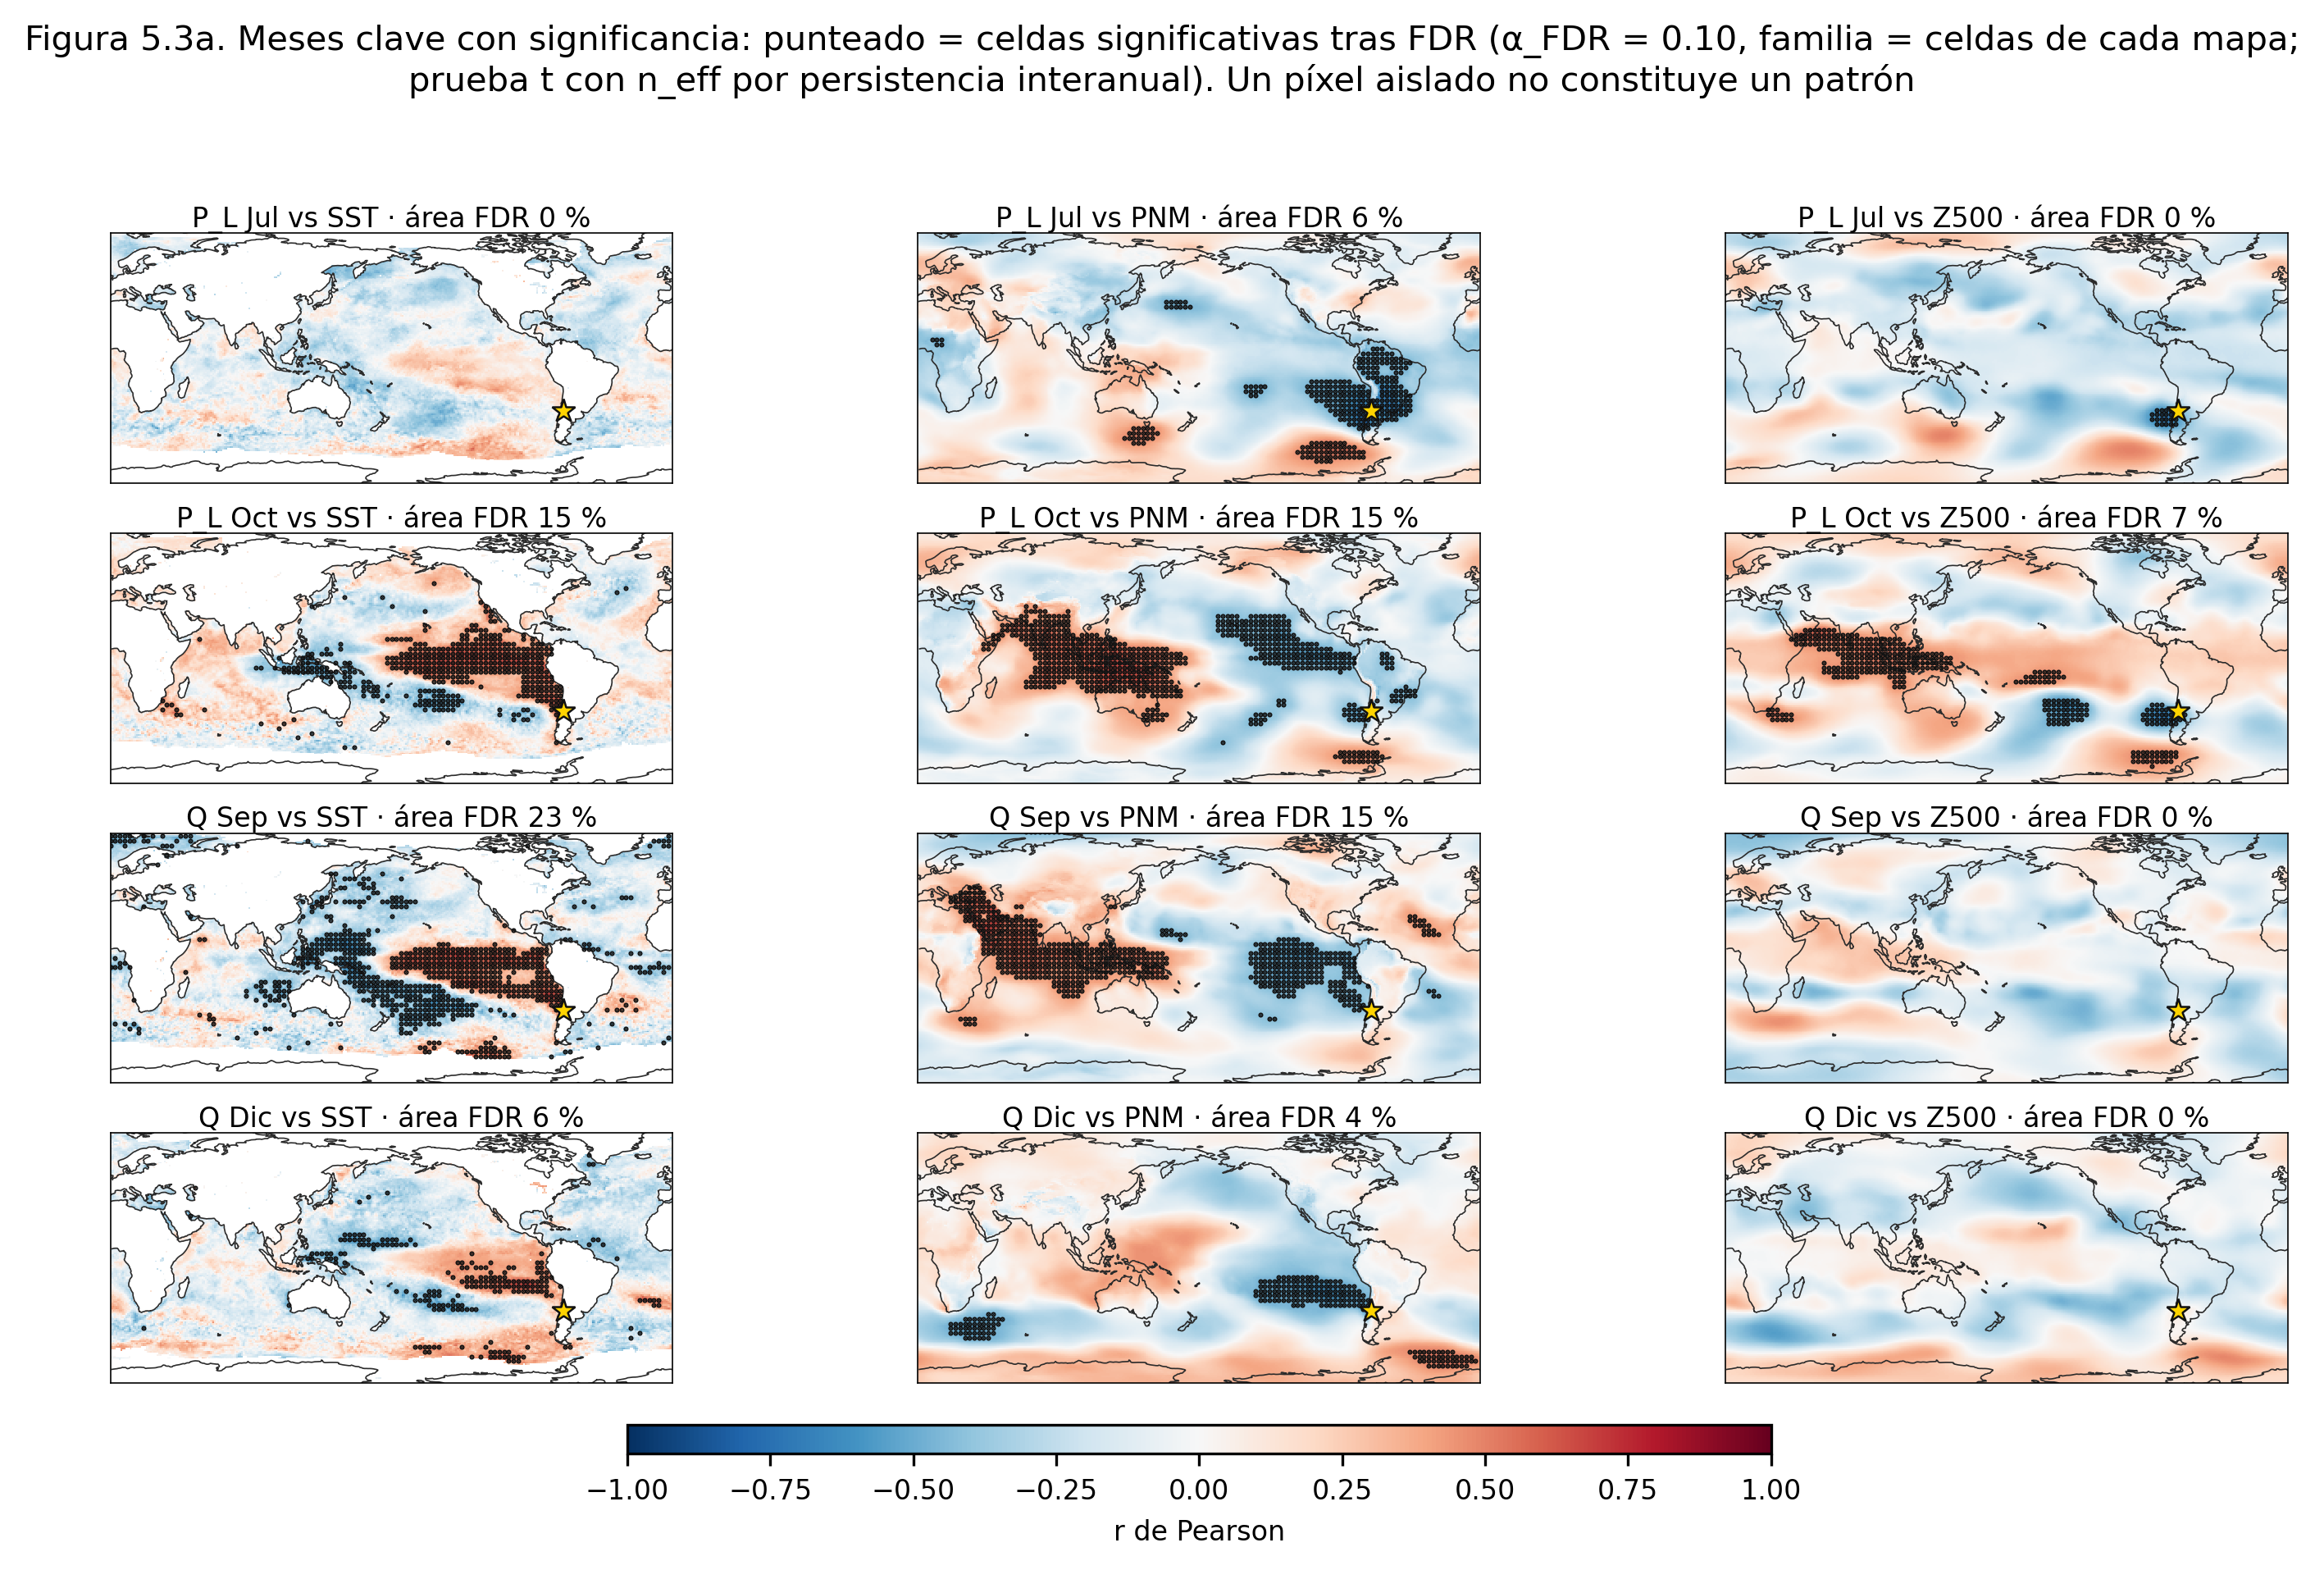
\includegraphics[width=0.95\textwidth]{figura_5_3a_significancia_fdr.png}
\caption{Versión del informe (figura 5.3a). En el dashboard se elige variable, campo y mes.}
\end{figure}

\paragraph{Qué mostrar.} Tres vistas, en este orden: (1) $P_L$ · PNM · julio; (2) $Q$ · SST · septiembre;
(3) $P_L$ · SST · octubre.

\paragraph{Cómo se lee.} Cada celda es la correlación entre, por ejemplo, los 40 julios de lluvia y los 40
julios de presión en esa celda. Azul indica que cuando ese campo está \emph{bajo} hay más agua en la cuenca;
rojo, que cuando está \emph{alto} hay más agua. Los puntos marcan las celdas que siguen siendo significativas
después de corregir por miles de pruebas (FDR).

\begin{guion}
``Correlacionamos cada mes de la cuenca con tres campos globales de ERA5, a lo largo de 40 años. En julio, la
lluvia se asocia con presión baja justo frente a Chile central, con correlaciones cercanas a menos 0.6: cuando
el anticiclón se debilita, los frentes llegan. El caudal muestra otra cosa: en septiembre aparece la forma de
herradura de El Niño en el Pacífico tropical, y el área significativa llega al 23\,\%. La lluvia también se
asocia con El Niño, pero sobre todo en octubre.''
\end{guion}

\begin{cifras}
\begin{itemize}
\item $P_L$--PNM local, abril--octubre: $r$ de $-0.38$ a $-0.64$; julio $-0.63$.
\item $Q$--SST en septiembre: 23\,\% del área significativa tras FDR; Niño 3.4 $r=0.63$.
\item $P_L$--Niño 3.4 en octubre: $r=0.62$; en pleno invierno solo 0.23--0.40.
\end{itemize}
\end{cifras}

\paragraph{Si te preguntan\ldots}
\begin{itemize}
\item \emph{¿Por qué estos tres campos?} SST por ENSO; PNM por el anticiclón que bloquea o deja pasar los frentes;
Z500 por las vaguadas y bajas segregadas en altura. Cada uno representa un eslabón del mecanismo.
\item \emph{¿Geopotencial o altura geopotencial?} ERA5 entrega el geopotencial en m$^2$/s$^2$; lo dividimos por
$g_0=9.80665$ para obtener la altura en metros.
\item \emph{¿Y el hielo?} ERA5 deja la SST bajo el hielo marino en el punto de congelación; esas celdas se
enmascararon junto con la tierra.
\end{itemize}

% -----------------------------------------------------------------------------
\section{Diapositiva 02 --- ¿En qué meses? (35 s)}

\begin{figure}[H]
\centering
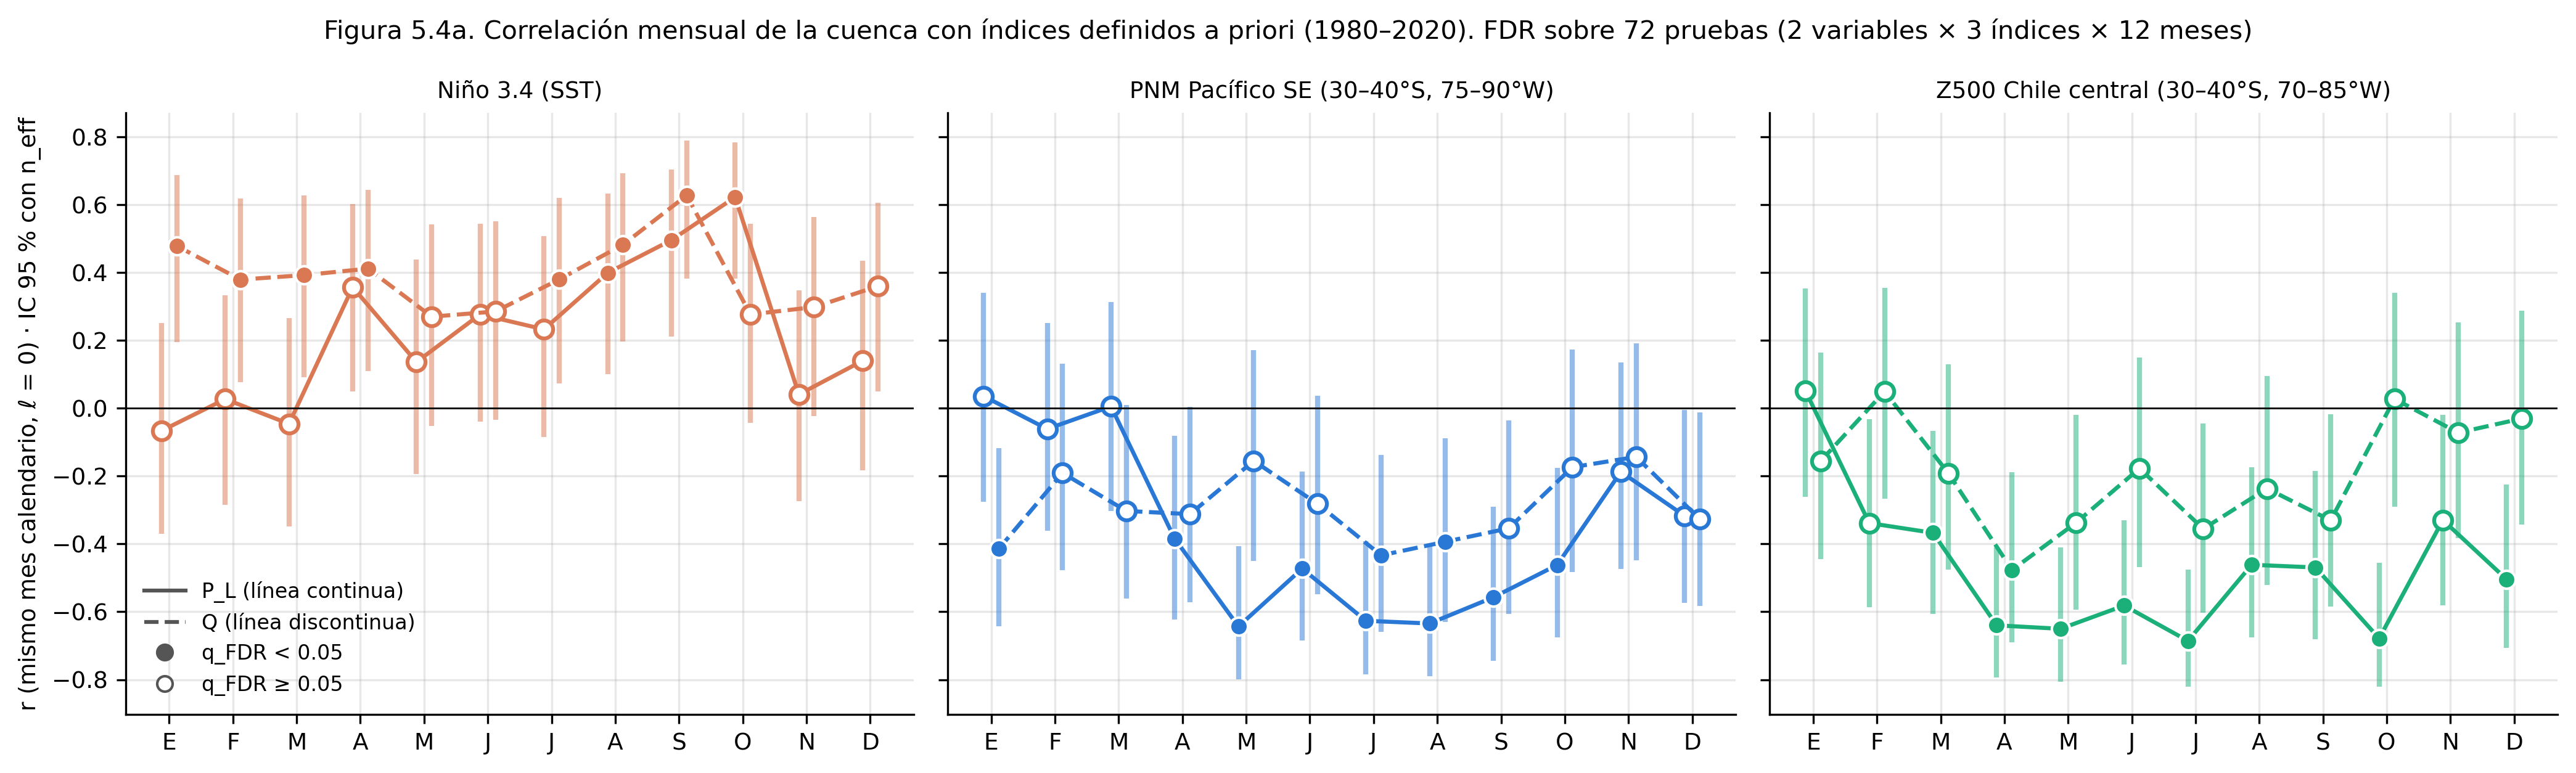
\includegraphics[width=\textwidth]{figura_5_4a_perfiles_indices.png}
\caption{Versión del informe (figura 5.4a).}
\end{figure}

\paragraph{Cómo se lee.} Para no elegir la celda más alta del mapa, que sería hacer trampa con el azar, se
definieron tres cajas \emph{antes} de mirar los mapas: Niño 3.4, la presión del Pacífico sureste y la Z500
sobre Chile central. Cada punto es la correlación de un mes; la barra, su intervalo del 95\,\%; el punto relleno,
significativo tras FDR.

\begin{guion}
``Con tres índices fijados de antemano, la lluvia se asocia con la presión y la Z500 locales en todos los meses de
abril a octubre, con correlaciones de menos 0.5 a menos 0.7. Es nuestro resultado más sólido. El Niño solo es
significativo de agosto a octubre, hacia el final de la estación lluviosa. Y el caudal se asocia con El Niño
todo el año, incluso en verano, cuando no llueve. Eso nos dice que algo guarda la señal.''
\end{guion}

\begin{cifras}
\begin{itemize}
\item 30 de 72 pruebas son significativas tras FDR; 16 son de $P_L$ con PNM o Z500.
\item $P_L$--Niño 3.4: agosto 0.40, septiembre 0.50, octubre 0.62. $Q$--Niño 3.4: 0.27--0.63, con 7 meses significativos.
\end{itemize}
\end{cifras}

% -----------------------------------------------------------------------------
\section{Diapositiva 03 --- ¿Es robusto? (35 s)}

\begin{figure}[H]
\centering
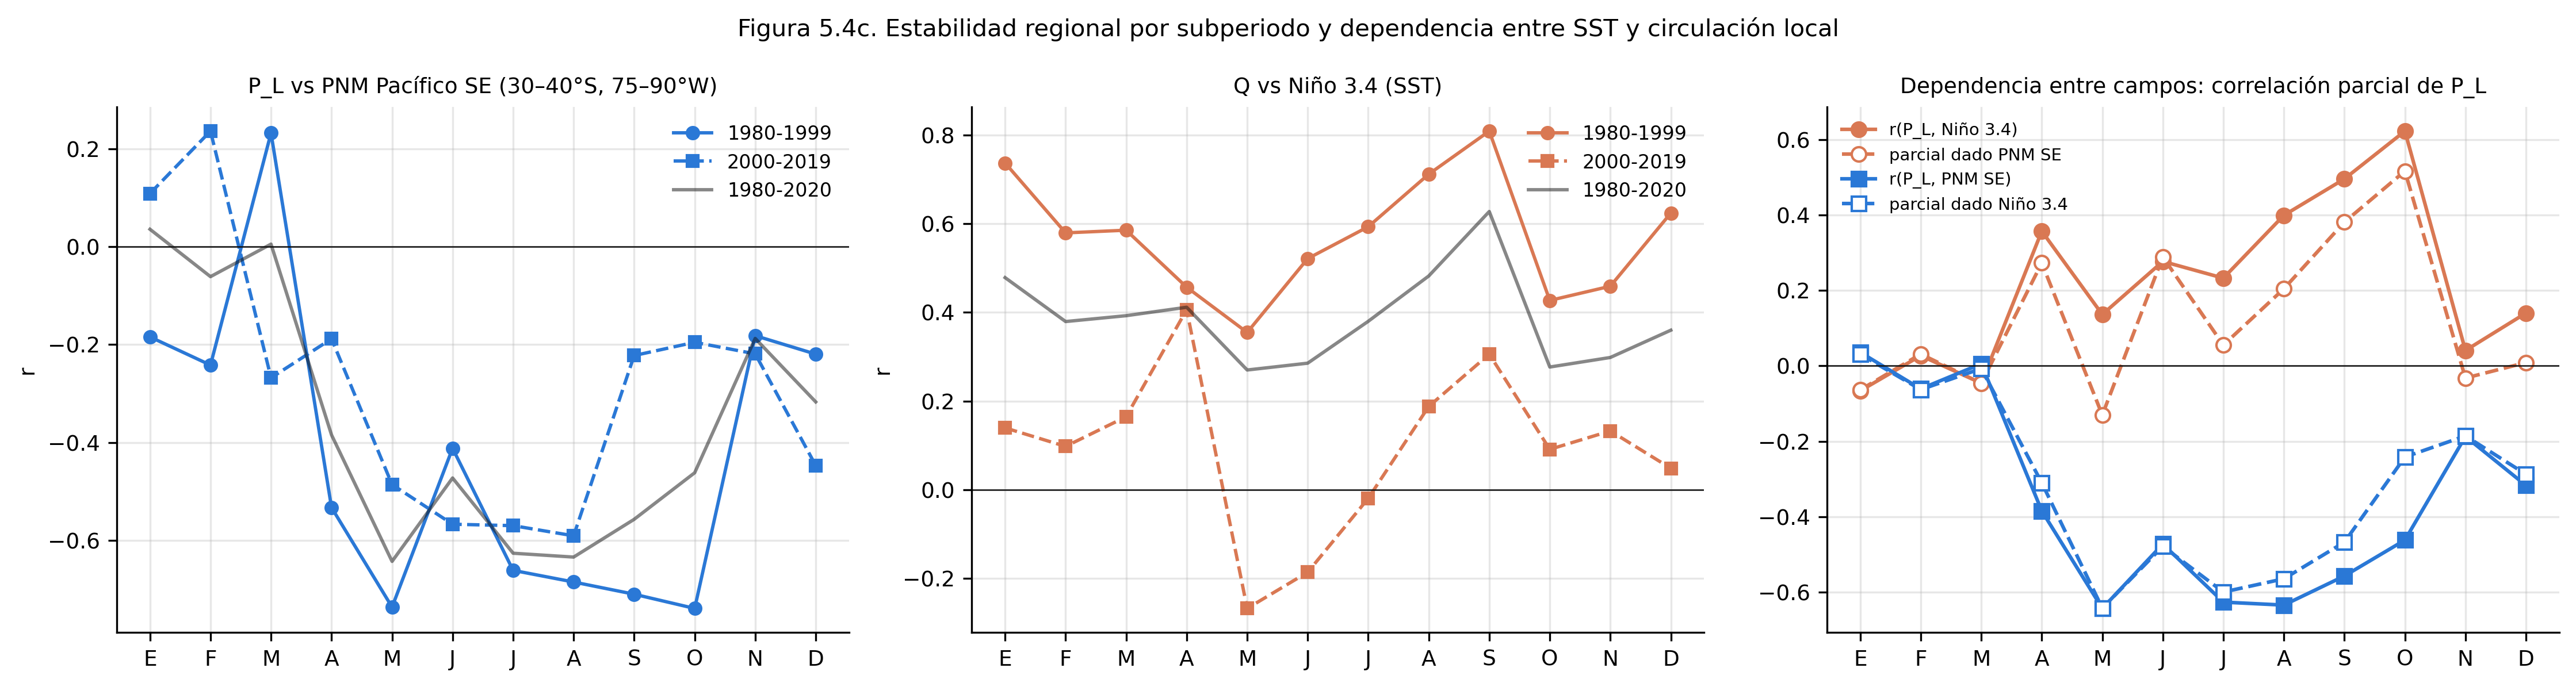
\includegraphics[width=\textwidth]{figura_5_4c_subperiodos_parcial.png}
\caption{Versión del informe (figura 5.4c); la estabilidad de los mapas está en la figura 5.3c.}
\end{figure}

\paragraph{Cómo se lee.} Los números a la derecha de la diapositiva comparan mapas completos: un 1 indica el
mismo patrón y menos de 0.3, que el patrón no se reproduce. La gráfica separa 1980--1999 (celeste) de
2000--2019 (naranja).

\begin{guion}
``Comprobamos que el resultado no lo producen las tendencias: al quitarlas, los mapas son prácticamente iguales.
Tampoco depende de los años extremos ni de la fuente, porque IMERG da los mismos patrones que la lluvia de
referencia. Pero al partir el registro en dos, la relación del caudal con El Niño cae de 0.8 a 0.3 en
septiembre. La relación de la lluvia con la presión local, en cambio, se mantiene en pleno invierno. La
teleconexión con ENSO no es estacionaria: se debilitó durante la megasequía.''
\end{guion}

\begin{cifras}
\begin{itemize}
\item Correlación entre patrones: con/sin tendencia 0.89--0.99; sin extremos 0.75--0.92; IMERG 0.82--0.86;
subperiodos 0.04--0.34.
\item $Q$--Niño 3.4 en septiembre: 0.81 (1980--1999) frente a 0.31 (2000--2019). $P_L$--PNM mayo--agosto: $-0.41$ a $-0.74$ frente a $-0.49$ a $-0.59$.
\end{itemize}
\end{cifras}

\paragraph{Si te preguntan\ldots}
\begin{itemize}
\item \emph{¿Cómo trataron la persistencia?} Con un tamaño de muestra efectivo por celda (Bretherton et al., 1999)
calculado con la autocorrelación entre años. En meses calendario resultó débil ($n_\mathrm{eff}\approx n$).
\item \emph{¿Qué familia usaron en el FDR?} Las celdas de cada mapa, con $\alpha_\mathrm{FDR}=0.10$, como
recomienda Wilks (2016) para campos espacialmente correlacionados. Por eso pedimos patrones, no píxeles sueltos.
\item \emph{¿Por qué cae la correlación después de 2000?} Hipótesis: en la megasequía la lluvia fue baja con
cualquier fase de ENSO; El Niño de 2015 no trajo lluvia (Garreaud et al., 2020). Con 20 años no se separa del
ruido.
\end{itemize}

% -----------------------------------------------------------------------------
\section{Diapositiva 04 --- ¿Qué mecanismo? (45 s) --- la más importante}

\begin{figure}[H]
\centering
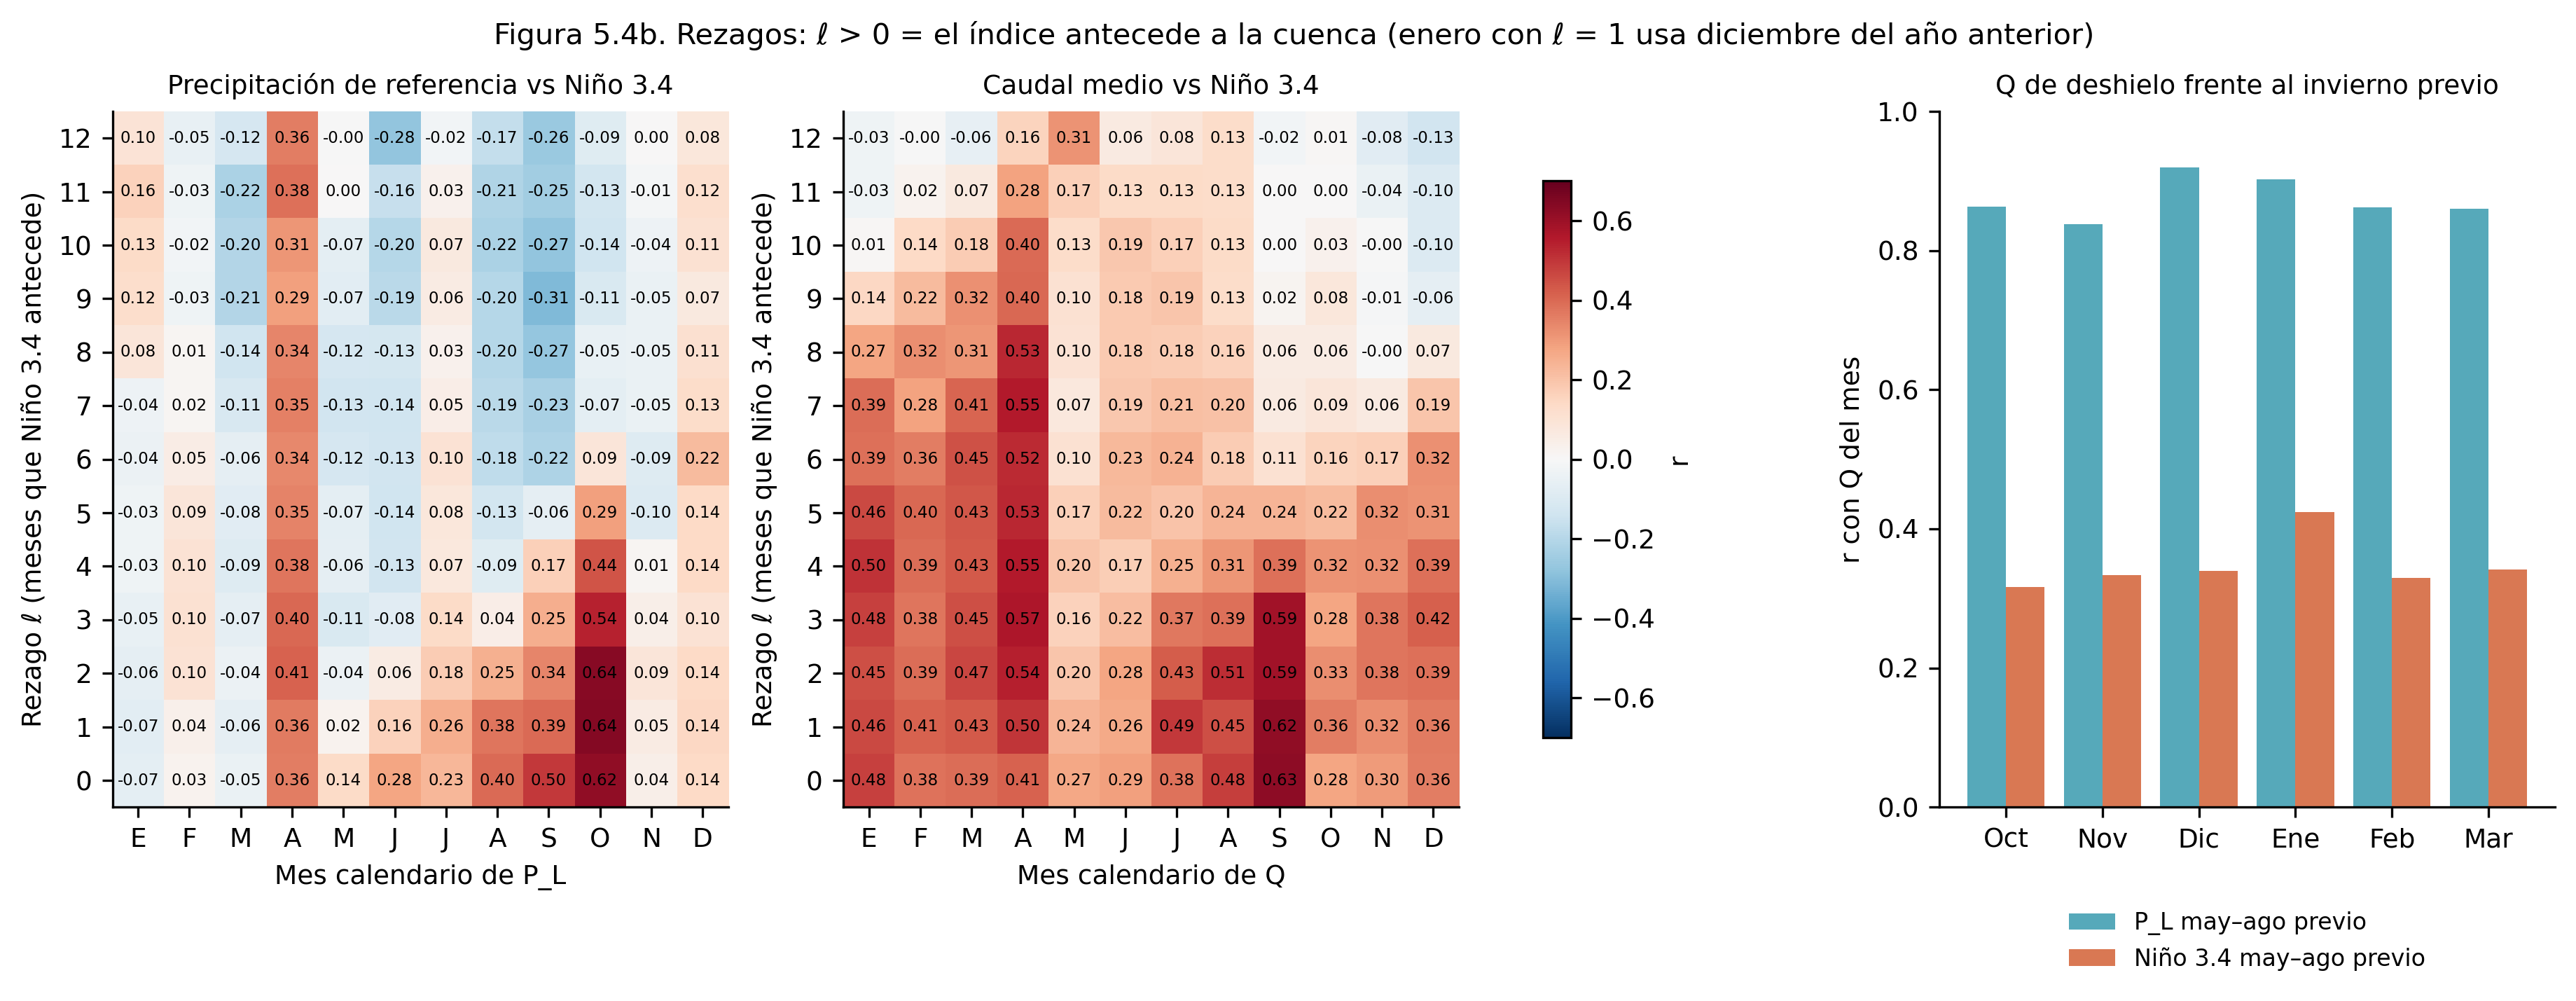
\includegraphics[width=\textwidth]{figura_5_4b_rezagos_nino34.png}
\caption{Versión del informe (figura 5.4b); la diapositiva muestra el panel derecho.}
\end{figure}

\paragraph{Cómo se lee.} Cada par de barras compara el caudal de un mes de la temporada de deshielo (octubre a
marzo) con lo que pasó el invierno anterior (mayo--agosto): la lluvia (celeste) y El Niño (naranja).

\begin{guion}
``Este es el mecanismo. El caudal de deshielo, de octubre a marzo, se explica casi por completo por la lluvia del
invierno anterior: correlaciones de 0.84 a 0.92. Es la memoria de la nieve que vimos en los puntos 1 y 4. Y ese
mismo caudal se asocia, más débilmente, con El Niño de ese invierno. La cadena es: El Niño debilita el
anticiclón, llueve más en invierno, se acumula más nieve y el río lleva más agua en verano. Además, al controlar
por la presión local, la correlación de la lluvia con El Niño en agosto baja de 0.40 a 0.20. ENSO actúa en buena
parte a través de esa circulación local. Pero la correlación simultánea no demuestra capacidad de pronóstico.''
\end{guion}

\begin{cifras}
\begin{itemize}
\item $Q$ (octubre--marzo) frente a $P_L$ de mayo--agosto: $r=0.84$--0.92. Frente a Niño 3.4 invernal: 0.32--0.42.
\item Correlación parcial: $P_L$--Niño 3.4 en agosto 0.40 $\rightarrow$ 0.20; $P_L$--PNM en julio $-0.63$ $\rightarrow$ $-0.60$.
\item Coherencia $Q$--Niño 3.4 en 2--7 años: media 0.27, máximo 0.49 cerca de 5 años (umbral 0.39).
\end{itemize}
\end{cifras}

\paragraph{Si te preguntan\ldots}
\begin{itemize}
\item \emph{¿Por qué un rezago de 6 meses?} Por la física de la cuenca: la nieve de invierno se derrite en verano
(desfase de 6--7 meses en los puntos 1 y 2). El mapa con $\ell=6$ (figura 5.2g) es más débil que el contemporáneo
porque Niño 3.4 persiste varios meses: la señal ya está en el mes simultáneo.
\item \emph{¿Se conecta con el punto 4?} Sí: el punto 4 no encontró un pico interanual robusto, y la coherencia con
ENSO es solo marginal. Compartir la banda de 2--7 años no prueba causalidad.
\end{itemize}

% -----------------------------------------------------------------------------
\section{Diapositiva 05 --- Síntesis (20 s)}

\begin{guion}
``En síntesis: lo más sólido es local, una presión baja frente a Chile en invierno. El Pacífico tropical modula esa
lluvia hacia fines del invierno y la nieve lleva su huella al caudal de verano, pero esa conexión se debilitó en
la megasequía. Por eso no hablamos de un ciclo ni de un pronóstico.''
\end{guion}

% -----------------------------------------------------------------------------
\section{Lo que NO debes decir}

\begin{itemize}
\item ``El Niño causa la lluvia del Maipo.'' Es una asociación; su efecto pasa en parte por la circulación local.
\item ``Con El Niño podemos pronosticar el caudal.'' No evaluamos pronóstico fuera de muestra.
\item ``Los puntos negros son las zonas que influyen.'' Son celdas significativas; lo relevante es el patrón coherente.
\item ``Hay un ciclo de ENSO en el caudal.'' La coherencia es marginal y el punto 4 no encontró un pico robusto.
\item ``El Modo Anular del Sur explica la megasequía.'' El dipolo de presión lo sugiere, pero no lo probamos.
\end{itemize}

\section{Decisiones de método en una línea}

\begin{table}[H]
\centering\small
\begin{tabularx}{\textwidth}{l X}
\toprule
Decisión & Justificación \\
\midrule
ERA5 a 1$^\circ$, 1979--2020 & Malla global moderada para patrones de gran escala; 1979 permite rezagos. \\
Correlación mes a mes a través de los años & Lo pide la guía; evita la asociación por el ciclo anual compartido. \\
Referencia de anomalías 2000--2020 & La misma de la cuenca; en un mes fijo no cambia Pearson. \\
Pearson y Spearman & Spearman por la asimetría de la lluvia; los patrones coinciden (0.72--0.99). \\
$n_\mathrm{eff}$ + FDR $\alpha=0.10$ por mapa & Persistencia y miles de pruebas; Wilks (2016). \\
Sin tendencia, subperiodos, sin extremos, IMERG & Robustez exigida en 5.3. \\
Cajas a priori & Evitan escoger la celda de mayor correlación. \\
\bottomrule
\end{tabularx}
\end{table}

\end{document}
